%!TEX root=../main.tex

\section{Introduction} % (fold)
\label{sec:introduction}

\cite{happMultivariateFunctionalPrincipal2018} develop innovative theory and methodology for the dimension reduction of multivariate functional data on possibly different dimensional domains (e.g., curves and images), which extends existing methods that were limited to either univariate functional data or multivariate functional data on a common one-dimensional domain. Recent research has shown a growing presence of data defined on different dimensional domains in diverse fields such as biomechanics, e.g., \cite{warmenhovenBivariateFunctionalPrincipal2019} and neuroscience, e.g., \cite{songSparseMultivariateFunctional2022}, so we expect the work to have significant practical impact. We aim to provide commentary on the estimation of the number of principal components utilising the methodology proposed in \cite{happMultivariateFunctionalPrincipal2018}. To achieve this, we conduct an extensive simulation study and subsequently propose practical guidelines for practitioners to adeptly choose the appropriate number of components for multivariate functional datasets. For ease of presentation, we use the same notation as in \cite{happMultivariateFunctionalPrincipal2018}. Code to reproduce the simulation study and data analysis in this discussion is available at \url{https://github.com/FAST-ULxNUIG/variance_mfpca}.

% section introduction (end)

\section{Model} % (fold)
\label{sec:model}

\cite{happMultivariateFunctionalPrincipal2018} proposed an extension of functional principal components analysis (FPCA, \cite{ramsayFunctionalDataAnalysis2005}) to multivariate functional data defined on different dimensional domains, named multivariate functional principal components analysis (MFPCA). We briefly present the estimation procedure of the principal components given a sample $x_1, \dots, x_N$ of multivariate functional data. The detailed estimation procedure is given in \cite{happMultivariateFunctionalPrincipal2018}, Section 3. For all $n = 1, \dots, N$, the observation $x_n$ is a vector of $p$ functions, each defined on a domain with possibly different dimensions. We denote by $x_n^{(j)}$ the $j$th entry of the vector $x_n$, referred to as the $j$th feature. The first step is to perform a univariate FPCA for each individual feature $j$ using $x_1^{(j)}, \dots, x_N^{(j)}$. We estimate $M_j$ univariate functional principal components for each feature $j$. The total number of components that have been estimated over all $p$ features is thus $M_+ = \sum_{j = 1}^p M_j$. We also define $M_{-} = \min_{j = 1, \dots, p} M_j$ to be the minimum number of univariate components estimated across all univariate features $j$. The univariate FPCA scores are estimated by projecting the (mean-centered) univariate functional observations onto the estimated eigenfunctions. The univariate scores from the $p$ features are then concatenated in a matrix of size $N \times M_+$. An eigenanalysis of this matrix is performed resulting in eigenvalues $\nu_m$ and eigenvectors $\mathbf{c}_m$. Finally, the multivariate eigenfunctions and scores are estimated as a linear combination of the univariate eigenfunctions and scores weighted by the eigenvectors $\mathbf{c}_m$. The multivariate eigenvalues are the same as the eigenvalues of the matrix of the concatenated scores $\nu_m$. In this context, our focus lies in investigating how the selection of the parameter $M_j$ impacts the estimation of the eigenvalues $\nu_m$.

Using this methodology, the maximum number of multivariate eigenvalues that can be estimated is $M_+$. Let $\{\nu_m\}_{1 \leq m \leq M_+}$ be the set of true eigenvalues and $\{\widehat{\nu}_m\}_{1 \leq m \leq M_+}$ be the set of estimated eigenvalues. We use the relative errors $\text{Err}(\widehat{\nu}_m)  = (\nu_m - \widehat{\nu}_m)^2 / \nu^2_m$ to assess the accuracy of the estimates. The authors also propose to estimate the number of multivariate components using the percentage of variance explained. For that, they first select $M_j$ univariate components that explain $\alpha\%$ of the variance for each univariate features \cite[Chapter 8.2]{ramsayFunctionalDataAnalysis2005} and they claim that this number of components is enough to estimate the number of multivariate components that explain $\alpha\%$ of the variance in the multivariate functional data \cite[Section 3.2]{happMultivariateFunctionalPrincipal2018}. The percentage of variance explained by the $m$th component and the cumulative percentage of variance explained by the first $m$ components are defined as
\begin{equation}\label{eq:pve}
     \text{PVE}_m = 100 \times \nu_m \times \left(\sum_{l = 1}^{M_+} \nu_l\right)^{-1} \quad\text{and}\quad \text{PVE}_{1:m} = \sum_{l = 1}^m \text{PVE}_l, \quad m = 1, \dots, M_+.
\end{equation}
If we fix the percentage of variance explained to be $\alpha\%$, the number of components needed to explain $\alpha\%$ of the variance is given by
\begin{equation}\label{eq:npc}
     \text{NPC}_{\alpha} = \sum_{m = 1}^{M_{+}} \mathbf{1}\left\{\text{PVE}_{1:m} < \alpha\right\} + 1.
\end{equation}


% section model (end)

\section{Simulation} % (fold)
\label{sec:simulation}

We perform a simulation study based on the first setting in the simulation in \cite{happMultivariateFunctionalPrincipal2018}. The data-generating process is based on a truncated version of the Karhunen-Loève decomposition. First, we generate a large orthonormal basis $\{\psi_m\}_{1 \leq k \leq M}$ of $\sLp{\TT{}}$ on an interval $\TT{} = [0, T] \subset \RR$. We fix $T_1 = 0$ and $T_{p + 1} = T$ and we generate $p - 1$ cut points $T_2, \dots, T_p$ uniformly in $\TT{}$ such that $0 = T_1 < \cdots < T_p < T_{p+1} = T$. Let $s_1, \dots, s_p \in \{-1, 1\}$ be coefficients that randomly flip the eigenfunctions with probability $0.5$, \textcolor{blue}{generated according to a Bernoulli distribution}. The univariate components of the eigenfunctions are then defined as
\begin{equation}\label{eq:simulation_uni_component}
    \psi_m^{(j)}(t_j) = s_j \restr{\psi_m}{[T_j, T_{j + 1}]}\left(\frac{t_j - T_j}{T_{j + 1} - T_j}\right), \quad m = 1, \dots, M, \quad j = 1, \dots, p.
\end{equation}
The notation $\restr{\psi_m}{[T_j, T_{j + 1}]}$ is the restriction of the function $\psi_m$ to the set $[T_j, T_{j + 1}]$. The set of multivariate functions $\{\psi_m\}_{1 \leq m \leq M}$ is an orthonormal system in $\HH \coloneqq \sLp{\TT{1}} \times \dots \times \sLp{\TT{p}}$ with $\TT{j} = [0, 1]$. Each curve is then simulated using the truncated multivariate Karhunen-Loève expansion,
\begin{equation}
    x_i(\pointt) = \sum_{m = 1}^M \rho_{i, m} \psi_m(\pointt), \quad \pointt \in \TT{},\quad i = 1, \dots, N,
\end{equation}
where the scores $\rho_{i, m}$ are sampled as Gaussian random variables with mean $0$ and variance $\nu_m$. The eigenvalues $\nu_m$ are defined with an exponential decrease, $\nu_m = \exp(-(m + 1)/2)$. We simulate $N = 25, 50$ and $100$ observations for each replication of the simulation. Similarly, each component is sampled on a regular grid of $S = 25, 50$ and $100$ sampling points. We use $p = 5$ features and we set $M = 50$. The estimation is done using the \textsf{R} package \texttt{MFPCA} (\cite{happ-kurzObjectOrientedSoftwareFunctional2020}). For each univariate feature $j$, we estimate $M_j$ principal components. Then, following the multivariate components estimation procedure, we can estimate $M_+$ multivariate components. The simulations are replicated $500$ times.

Figure \ref{fig:ncomp} displays a comparison of the error in the estimated eigenvalues when using $M_j = 5$ and $M_j = 10$, illustrating the effect of $M_j$ on eigenvalue estimation. The accuracy of the estimation declines with an increasing number of components in all scenarios. In particular, there is a notable jump in accuracy observed for the last five estimated eigenvalues when $M_j = 5$, while this is not clear when $M_j = 10$. The dependence of the eigenvalue estimates on the number of univariate functional principal components retained $M_j$ is clear, but establishing a general rule based on these observations is challenging. We suggest to estimate at most $M_{-}$ multivariate components; otherwise, the univariate components may not contain enough information to effectively recover their corresponding multivariate counterparts.
\begin{figure}
     \centering
    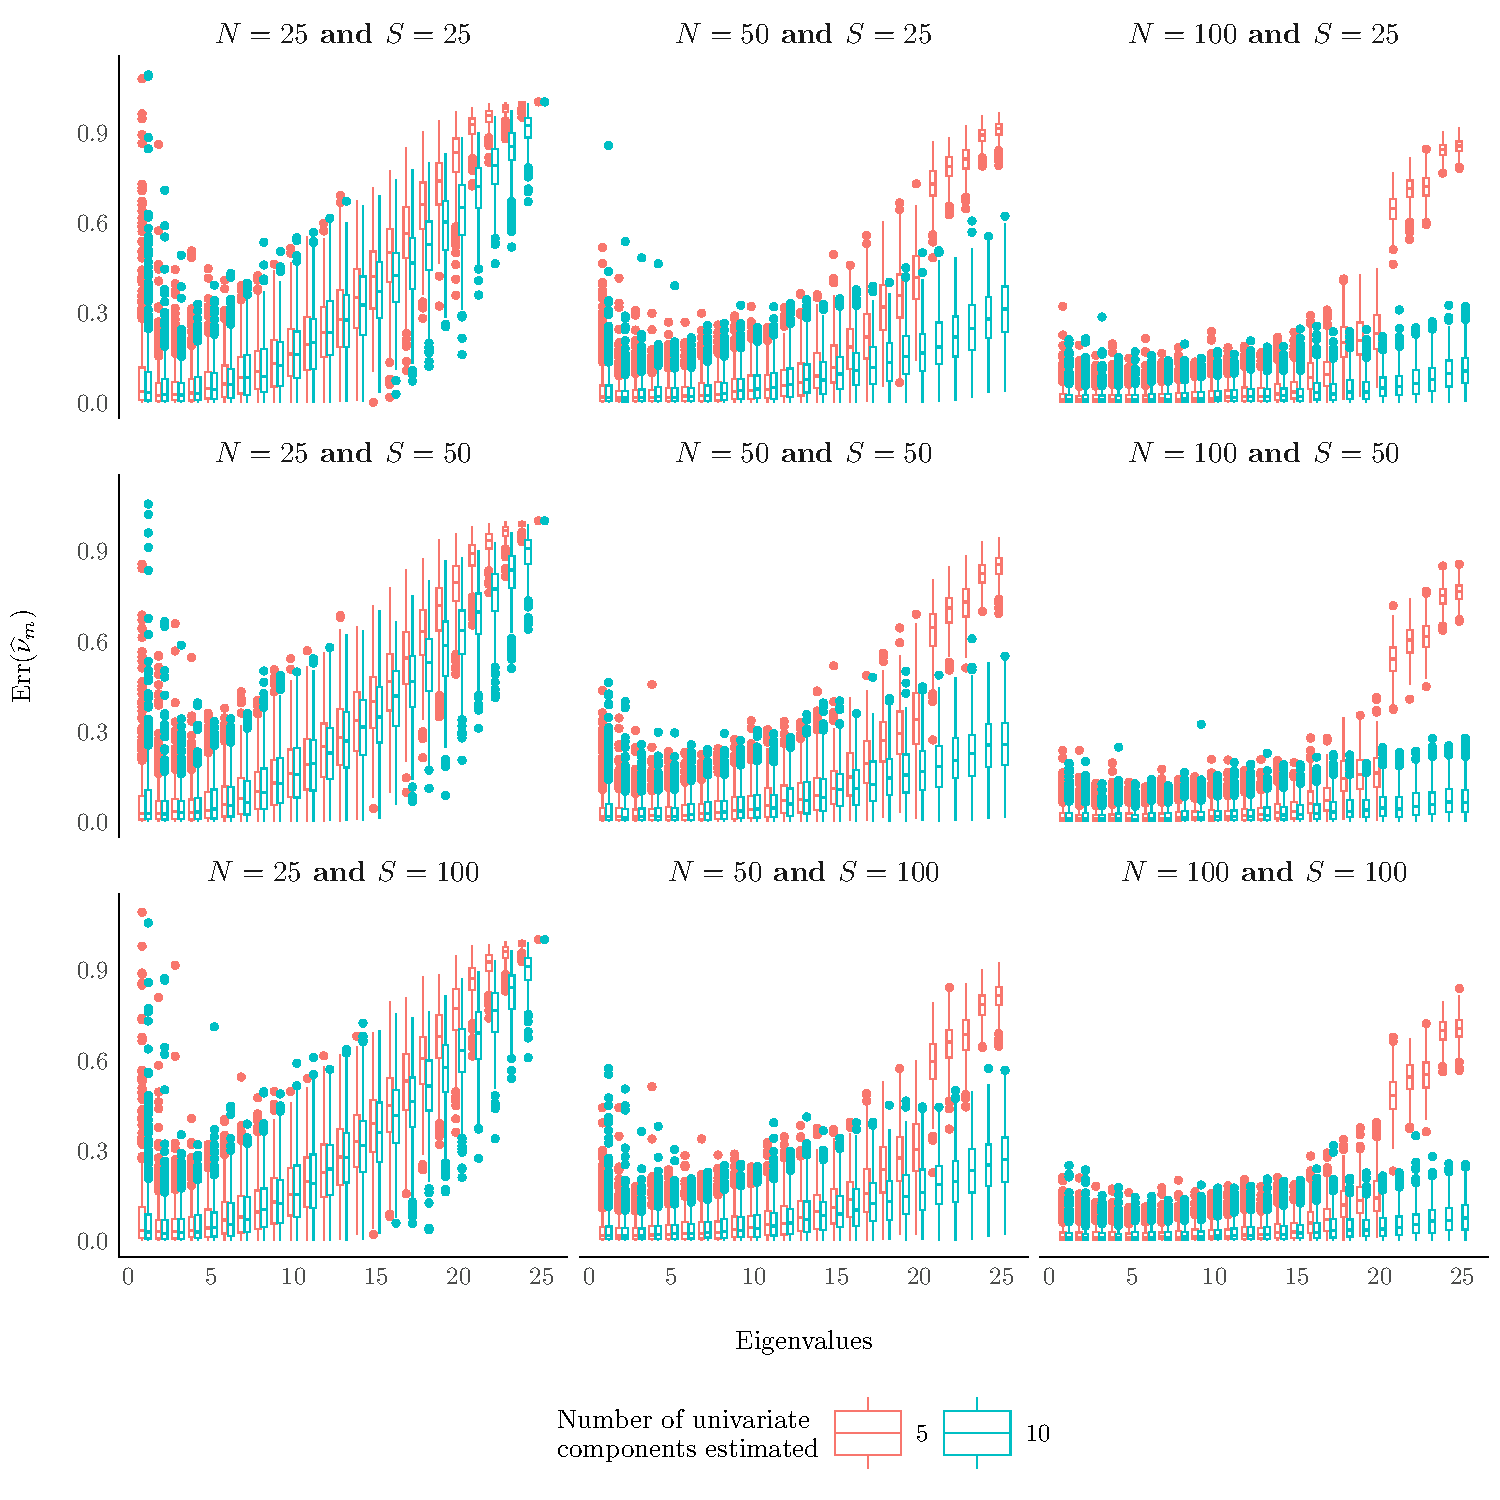
\includegraphics[width=0.94\textwidth]{figures/ncomp.pdf}
    \caption{Boxplots of the estimation errors of the eigenvalues. We estimated $5$ (red boxplots) and $10$ (blue boxplots) univariate functional components for each of $p = 5$ univariate features. The number of multivariate eigencomponents that are estimated is $25$. $N$ is the number of observations, $S$ is the number of sampling points per curve. We run $500$ simulations.}
    \label{fig:ncomp}
\end{figure}
Figure \ref{fig:npc_estim} presents the estimation of the number of multivariate components retained across $500$ simulation scenarios for a fixed percentage of variance explained. The red dots represent the number of multivariate components that would be needed to explain at least $\alpha\%$ of the variance ($50\%, 70\%, 90\%, 95\%$ and $99\%$), considering an exponential decay of the eigenvalues as defined in equation \eqref{eq:npc}. Note that, we can compute the number of multivariate components exactly as we know the true eigenvalues. Additionally, the size of the black dots indicates the frequency of selection for each number of multivariate component over the $500$ simulations. For example, for the panel where $N = 25$ and $S = 25$, and for a proportion of variance explained $\alpha = 0.5$, for approximately $200$ simulations of the $500$, two multivariate components were selected and for around $300$ simulations of the $500$ only one multivariate component was selected to explain $50\%$ of the variance, while the true number of multivariate components is $2$ (red dot). Notably, the number of components appears to be consistently underestimated for various combinations of the number of observations $N$, number of sampling points $S$, and desired percentage of variance explained $\alpha\%$. Therefore, this simulation scenario shows that using a percentage of variance explained of level $\alpha$ to choose the number of univariate components $M_j$ is not sufficient to estimate the number of multivariate functional principal components that explain $\alpha\%$ of the variance in the multivariate functional data. These findings may hold considerable significance for practitioners.
\begin{table}
\begin{subtable}[h]{0.3\textwidth}
\centering
\begin{tabular}{rr|rr}
    & & \multicolumn{2}{c}{$\widehat{\text{NPC}}_{\alpha}$} \\
    $N$ & $S$ & 1 & 2 \\
    \hline
    25 & 25 & \textbf{301} & 199 \\
    25 & 50 & \textbf{276} & 224 \\
    25 & 100 & \textbf{270} & 230 \\
    50 & 25 & 235 & \textbf{265} \\
    50 & 50 & 208 & \textbf{292} \\
    50 & 100 & 254 & \textbf{246} \\
    100 & 25 & 158 & \textbf{342} \\
    100 & 50 & 165 & \textbf{335} \\
    100 & 100 & 178 & \textbf{322} \\
\end{tabular}
\caption{$\alpha = 50\%$ ($\text{NPC}_{\alpha} = 2$)}
\end{subtable}
\hfill
\begin{subtable}[h]{0.3\textwidth}
\centering
\begin{tabular}{rr|rrr}
    & & \multicolumn{3}{c}{$\widehat{\text{NPC}}_{\alpha}$} \\
    $N$ & $S$ & 1 & 2 & 3\\
    \hline
    25 & 25 & 1 & \textbf{464} & 35\\
    25 & 50 & 1 & \textbf{456} & 43\\
    25 & 100 & 1 & \textbf{461} & 38\\
    50 & 25 & 0 & \textbf{459} & 41\\
    50 & 50 & 0 & \textbf{461} & 39\\
    50 & 100 & 1 & \textbf{450} & 49\\
    100 & 25 & 0 & \textbf{467} & 33\\
    100 & 50 & 0 & \textbf{469} & 31\\
    100 & 100 & 0 & \textbf{471} & 29\\
\end{tabular}
\caption{$\alpha = 70\%$ ($\text{NPC}_{\alpha} = 3$)}
\end{subtable}
\hfill
\begin{subtable}[h]{0.3\textwidth}
\centering
\begin{tabular}{rr|rrr}
    & & \multicolumn{3}{c}{$\widehat{\text{NPC}}_{\alpha}$} \\
    $N$ & $S$ & 3 & 4 & 5 \\
    \hline
    25 & 25 & 15 & \textbf{400} & 85\\
    25 & 50 & 18 & \textbf{375} & 107\\
    25 & 100 & 12 & \textbf{379} & 109\\
    50 & 25 & 0 & \textbf{322} & 178\\
    50 & 50 & 0 & \textbf{271} & 229\\
    50 & 100 & 0 & \textbf{268} & 232\\
    100 & 25 & 0 & 212 & \textbf{288}\\
    100 & 50 & 0 & 157 & \textbf{343}\\
    100 & 100 & 0 & 136 & \textbf{364}\\
\end{tabular}
\caption{$\alpha = 90\%$ ($\text{NPC}_{\alpha} = 5$)}
\end{subtable}
\\
\begin{subtable}[h]{0.45\textwidth}
\centering
\begin{tabular}{rr|rrrr}
    & & \multicolumn{4}{c}{$\widehat{\text{NPC}}_{\alpha}$} \\
    $N$ & $S$ & 4 & 5 & 6 & 7 \\
    \hline
    25 & 25 & 6 & \textbf{379} & 115 & 0\\
    25 & 50 & 5 & \textbf{376} & 118 & 1\\
    25 & 100 & 1 & \textbf{357} & 142 & 0\\
    50 & 25 & 0 & \textbf{288} & 212 & 0\\
    50 & 50 & 0 & 232 & \textbf{267} & 1\\
    50 & 100 & 0 & 210 & \textbf{289} & 1\\
    100 & 25 & 0 & 172 & \textbf{328} & 0\\
    100 & 50 & 0 & 110 & \textbf{390} & 0\\
    100 & 100 & 0 & 84 & \textbf{416} & 0\\
\end{tabular}
\caption{$\alpha = 95\%$ ($\text{NPC}_{\alpha} = 6$)}
\end{subtable}
\hfill
\begin{subtable}[h]{0.45\textwidth}
\centering
\begin{tabular}{rr|rrrr}
    & & \multicolumn{4}{c}{$\widehat{\text{NPC}}_{\alpha}$} \\
    $N$ & $S$ & 7 & 8 & 9 & 10\\
    \hline
    25 & 25 & 10 & \textbf{365} & 125 & 0\\
    25 & 50 & 2 & \textbf{362} & 136 & 0\\
    25 & 100 & 2 & \textbf{338} & 160 & 0\\
    50 & 25 & 0 & 117 & \textbf{383} & 0\\
    50 & 50 & 0 & 86 & \textbf{413} & 1\\
    50 & 100 & 0 & 52 & \textbf{448} & 0\\
    100 & 25 & 0 & 8 & \textbf{492} & 0\\
    100 & 50 & 0 & 0 & \textbf{499} & 1\\
    100 & 100 & 0 & 2 & \textbf{497} & 1\\
\end{tabular}
\caption{$\alpha = 99\%$ ($\text{NPC}_{\alpha} = 10$)}
\end{subtable}
\caption{\textcolor{blue}{Estimation of the number of components to explain $\alpha\%$ of the variance over $500$ simulations. The true number of components that explain $\alpha\%$ of the variance is given in parenthesis. $N$ is the number of observations, $S$ is the number of sampling points per curve.}}
\label{fig:npc_estim}
\end{table}


% section simulation (end)

\section{Application: Canadian weather dataset} % (fold)
\label{sec:application_canadian_weather_dataset}

To illustrate our simulation results, we apply the same idea on a real dataset, the Canadian weather dataset, available in the \textsf{R} package \texttt{fda} \citep{ramsayFdaFunctionalData2023}. The dataset contains daily measurements of temperature (in Celsius) and precipitation (in millimeters) for $35$ Canadian weather stations, averaged over the years 1960 to 1994. This is an example of multivariate functional data with $p = 2$ defined on one dimensional domain, the temperature being the first feature and the precipitation being the second feature. We aim to estimate $M$ multivariate eigencomponents of the data using different number of univariate eigencomponents and compare the results. For that, we define two scenarios, one where $M = M_{+}$ and one where $M = M_{-}$.

We first expand the data in a B-splines basis with $10$ functions. In the first scenario, for each feature, we estimate two univariate eigencomponents ($M_1 = 2$ and $M_2 = 2$). In the second scenario, for each feature, we estimate four univariate eigencomponents ($M_1 = 4$ and $M_2 = 4$). In both scenarios, we then estimate $M = 4$ multivariate eigencomponents. So, for the first scenario, $M = M_{+} = 4$ and for the second scenario, $M = M_{-} = 4$. Based on the simulation and Figure \ref{fig:ncomp}, we expect the first two multivariate eigencomponents to be similar and the other two to be unequal.

Table \ref{tab:eigenvalues} presents the estimation of the eigenvalues for the Canadian weather dataset for both scenarios. We notice that the values are similar for the first two eigenvalues, but quite different for the other two. 

\begin{table}[!h]
\centering
\begin{tabular}{c c | c c c c}
 & & \multicolumn{4}{c}{Eigenvalues} \\
Scenario & Univariate expansions & 1st & 2nd & 3rd & 4th \\
\hline
1 & $2$ components & $15845$ & $1675$ & $308$ & $45$ \\
2 & $4$ components & $15850$ & $1679$ & $438$ & $213$ \\
\hline
\end{tabular}
\caption{Estimation of the first four eigenvalues of the Canadian weather dataset using two and four univariate components for the univariate expansions.}
\label{tab:eigenvalues}
\end{table}

Figure \ref{fig:eigenfunctions_weather} presents the estimation of the eigenfunctions for the Canadian weather dataset for both scenarios. As with the eigenvalues, we notice that the first two (multivariate) eigenfunctions are approximately the same, but the other two are not equal. While we do not know the true eigenfunctions, based on simulation results, the estimated multivariate eigenfunctions from the second scenario should be closer to the truth than the estimation from the first scenario. We may explain this result as we have not estimated enough information in the univariate decomposition in the first scenario to effectively estimate the third and fourth multivariate eigencomponents. We reiterate the suggestion to estimate at most $M_{-}$ multivariate eigencomponents (which will be $M_{-} = 2$ for the first scenario).

\begin{figure}[!h]
     \centering
     \begin{subfigure}[b]{0.49\textwidth}
         \centering
         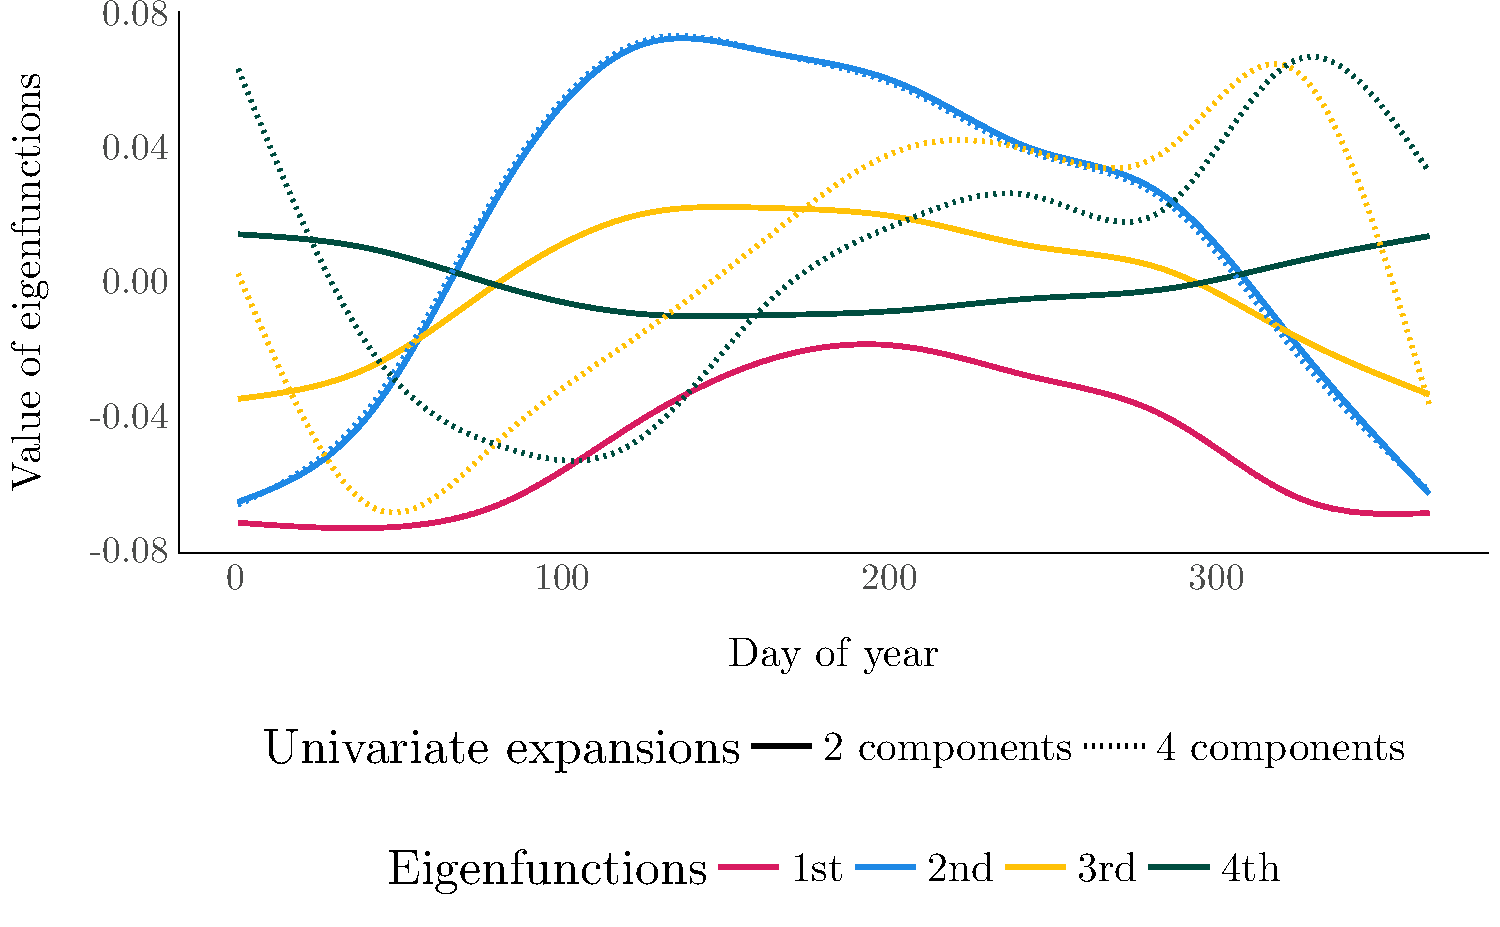
\includegraphics[width=1\textwidth]{figures/temperature_eigen.pdf}
         \caption{Temperature (first component)}
         \label{fig:temperature}
     \end{subfigure}
     \hfill
     \begin{subfigure}[b]{0.49\textwidth}
         \centering
         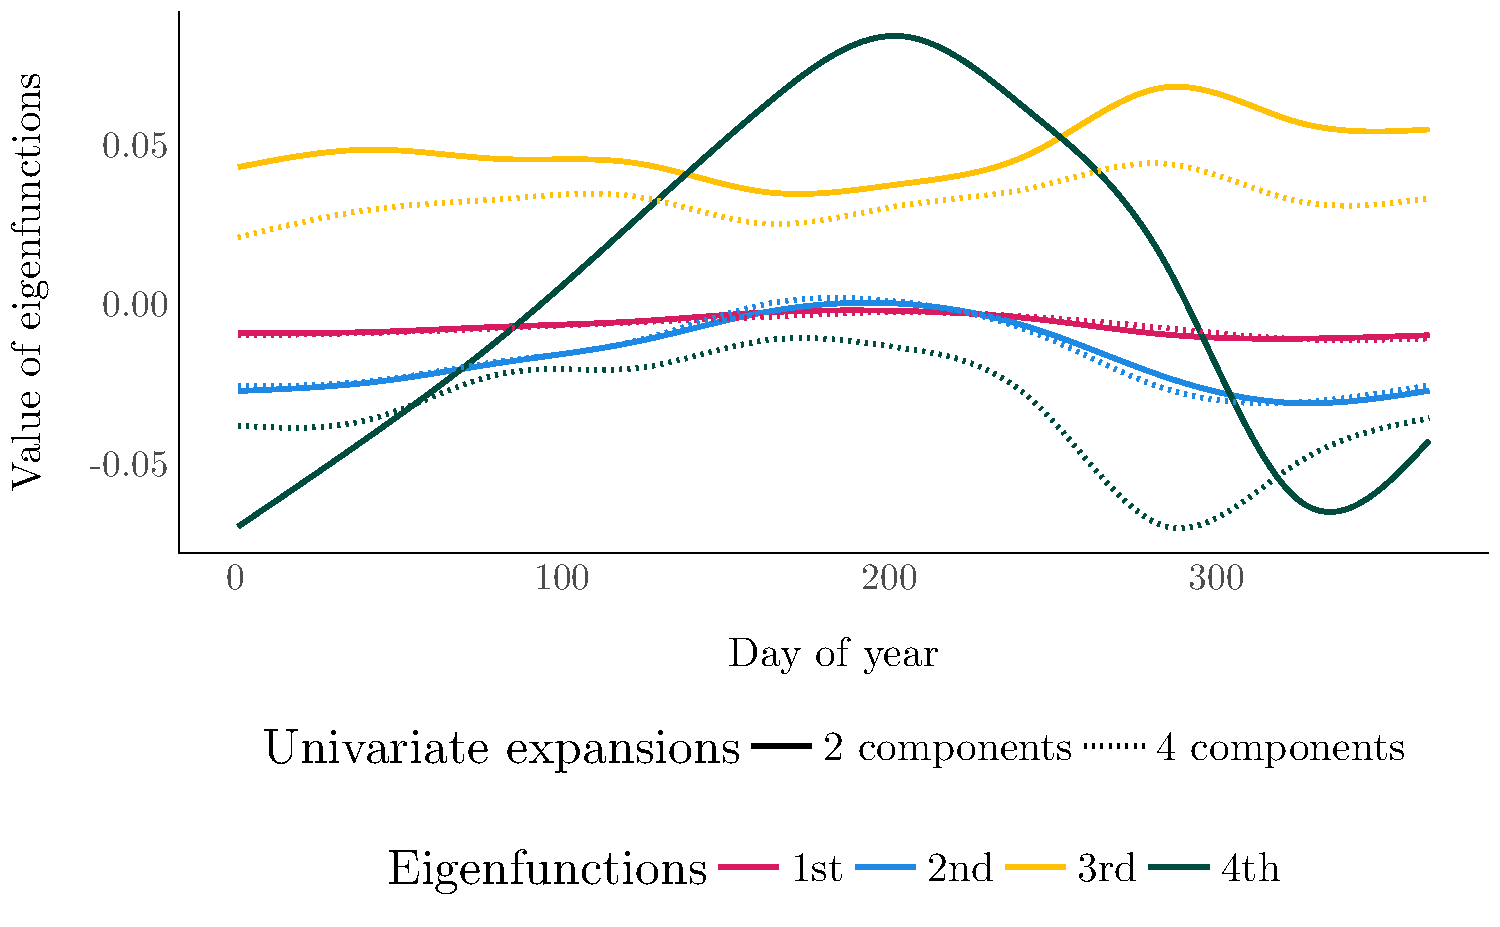
\includegraphics[width=1\textwidth]{figures/precipitation_eigen.pdf}
         \caption{Precipitation (second component)}
         \label{fig:precipitation}
     \end{subfigure}
     \caption{Estimation of the first four eigenfunctions of the Canadian weather dataset using using two and four univariate components for the univariate expansions.}
     \label{fig:eigenfunctions_weather}
\end{figure}

% section application_canadian_weather_dataset (end)

\section{Conclusion} % (fold)
\label{sec:conclusion}

\cite{happMultivariateFunctionalPrincipal2018} present a general methodology to estimate principal components for a set of multivariate functional data defined on, possibly, different dimensional domains. Their approach, based on the decomposition of the covariance of each univariate feature, allows easy estimation of the components.

We have conducted a simulation study and an example on a real dataset, and the obtained results highlight two important findings. Firstly, although utilizing only a few univariate components may yield a substantial number of multivariate components, their accuracy is notably limited. Secondly, relying on the percentage of variance explained as a criterion for selecting the number of univariate components may result in an underestimation of the number of multivariate components. We, therefore, advise practitioners to exercise caution when determining the number of estimated components required in their analysis. We suggest to estimate at most $M_{-}$ multivariate components. Additionally, we strongly recommend conducting simulations that closely resemble the characteristics of the actual data to select the appropriate number of components based on the percentage of variance explained criterion.

% section conclusion (end)





